% The document shown in the App Store screenshots. Build with:
%   pdflatex showcase.tex && pdflatex showcase.tex
\documentclass[11pt]{article}
\usepackage[paperwidth=5.5in,paperheight=8.5in,margin=0.55in]{geometry}
\usepackage[T1]{fontenc}
\usepackage{lmodern,microtype,amsmath,booktabs,tikz,pgfplots,xcolor}
\pgfplotsset{compat=1.18}
\usepackage[colorlinks=true,linkcolor=teal!70!black,urlcolor=teal!70!black,bookmarks=true,bookmarksopen=true]{hyperref}
\hypersetup{pdftitle={How Owls See in the Dark},pdfauthor={NightPdf}}
\setlength{\parskip}{0.35em}

\title{\textbf{How Owls See in the Dark}\\[0.3em]\large A field guide to nocturnal vision}
\author{Notes for curious night readers}
\date{}

\begin{document}
\maketitle
\vspace{-1.5em}
\tableofcontents

\section{Introduction}
Most birds go to sleep when the sun does. Owls go to work. Over millions of
years they have refined a set of adaptations that let them find a mouse in a
field on a moonless night, and many of those adaptations begin with the eye.

An owl's eyes are so large relative to its skull that they cannot rotate in
their sockets. Instead of moving its eyes, an owl moves its head, turning it
as much as 270 degrees. What it gives up in eye movement, it gains in light:
a bigger eye gathers more photons, and photons are the scarcest resource at
night.

This guide walks through the main ideas: how the eye collects light, how the
retina turns it into a signal, and how hearing fills in what the eyes cannot.

\section{Gathering Light}
The amount of light an eye collects depends on the area of its pupil. Doubling
the pupil diameter quadruples the light. Optical designers summarize this with
the \emph{f-number}, the ratio of focal length $f$ to aperture diameter $D$:
\begin{equation}
  N = \frac{f}{D}, \qquad E \propto \frac{1}{N^{2}},
\end{equation}
where $E$ is the brightness of the image on the retina. A tawny owl's eye has an
f-number near $1.3$, compared with about $2.1$ for a human eye in the dark.
That difference alone makes the owl's retinal image roughly two and a half
times brighter.

The eye is also tubular rather than round. This shape keeps a long focal length,
for a large image, without the weight of a full sphere. The trade-off is a
narrower field of view, which the owl recovers by turning its head.

\section{The Retina}
Light that reaches the retina is absorbed by two kinds of cells. \emph{Cones}
handle color and fine detail in bright light. \emph{Rods} are far more sensitive
and do most of the work at night. Owl retinas are dominated by rods.

\begin{center}
\small
\begin{tabular}{@{}lcc@{}}
\toprule
 & Human & Tawny owl \\
\midrule
Rods per cone       & 20 : 1   & 30 : 1 \\
Pupil f-number      & 2.1      & 1.3 \\
Head rotation       & 80$^\circ$ & 270$^\circ$ \\
\bottomrule
\end{tabular}
\end{center}

Behind the retina, many nocturnal animals have a reflective layer that sends
light back through the rods for a second chance at absorption. It is why a
flashlight makes their eyes shine. Owls rely less on this trick than cats do,
and more on sheer eye size.

\section{Sensitivity at Night}
Sensitivity grows as light fades, because the eye slowly adapts. Rods take
around thirty minutes to reach full sensitivity, which is why a dark room seems
to brighten the longer you sit in it.

\begin{center}
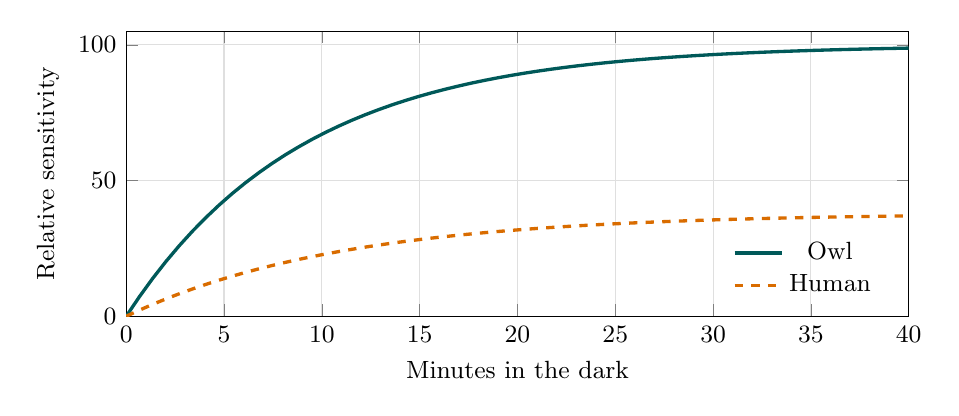
\begin{tikzpicture}
\begin{axis}[
  width=0.95\linewidth, height=5.2cm,
  xlabel={Minutes in the dark}, ylabel={Relative sensitivity},
  xmin=0, xmax=40, ymin=0, ymax=105,
  legend pos=south east, legend style={font=\small, draw=none, fill=none},
  grid=major, grid style={gray!25}, tick label style={font=\small},
  label style={font=\small}]
\addplot[very thick, teal!70!black, domain=0:40, samples=60]
  {100*(1-exp(-x/9))};
\addlegendentry{Owl}
\addplot[very thick, orange!85!black, dashed, domain=0:40, samples=60]
  {38*(1-exp(-x/11))};
\addlegendentry{Human}
\end{axis}
\end{tikzpicture}
\end{center}

The curves are illustrative, but the shape is real: a fast early rise as cones
adapt, then a slower climb as rods take over.

\section{Hearing the Unseen}
On the darkest nights even an owl's eyes are not enough, and it hunts by ear.
In barn owls the ear openings sit at different heights on each side of the
head. A sound from below reaches one ear slightly sooner and louder than the
other, so the owl can locate prey in both direction and elevation.

The facial disc, the ring of stiff feathers around the face, works like a
satellite dish. It funnels sound toward the ears, and the owl can reshape it
with small muscles to focus on what it is listening to.

\section{Silent Flight}
Hearing well is only useful if the hunter is quiet. Owl feathers have a comb of
fine serrations on their leading edge and a soft fringe on the trailing edge.
Together they break up the turbulence that makes a pigeon's wings whistle, so an
owl can glide in almost without a sound.

\section{Conclusion}
Night vision in owls is not one trick but a system: big tubular eyes with wide
apertures, rod-rich retinas, a head that turns to make up for fixed eyes, ears
that map sound in three dimensions, and feathers that keep the approach silent.

Reading at night, we borrow a little of the same idea. Dimming the page lets our
own eyes stay adapted to the dark, so the room around us stays visible and the
text stays comfortable.

\end{document}
